\documentclass[12pt]{report}

% Font and text formatting packages
\usepackage{microtype} % Improved text alignment and spacing
\usepackage[bitstream-charter]{mathdesign}
\usepackage{XCharter} % XCharter font
\usepackage[scaled]{beramono} % Monospaced font styling
% \usepackage[italic]{mathastext} % Italicizes math in text font for consistency

% Conditional checking
\usepackage{etoolbox}

% Enhanced typography
\usepackage[normalem]{ulem} % Underlining
\usepackage{contour} % Outline text (used with \contour command)
\usepackage{xpatch} % Enables patching commmands for typographical modifications
\usepackage{bm} % Italic bold

% Scientific notation and chemical formulas
\usepackage[version=4]{mhchem} % For chemical notation
\usepackage{siunitx} % Consistent handling of units

% Graphics
\usepackage{graphicx} % Essential for including images
\usepackage{subcaption} % Subfigures and subcaptions
\graphicspath{{./images/}} % Path for images directory

% Document layout
\usepackage[margin=1in]{geometry} % 1-inch margins
\usepackage{multicol} % Multi-column layouts

% Custom captions formatting
\usepackage{caption}
\DeclareCaptionFormat{custom}{\textbf{#1.} #3}
\captionsetup{format=custom}


\usepackage{csquotes} % Recommended for quotes in citations
\usepackage[style=apa, backend=biber]{biblatex} % APA style citations
\addbibresource{references.bib} % Reference file


% Custom underlining with contour effect
\contourlength{1.7pt} % Default contour length
\NewDocumentCommand{\ul}{O{2.62pt} O{0.45pt} O{1.5pt} m}{%
  \begingroup%
  \renewcommand\ULdepth{#1}%
  \renewcommand\ULthickness{#2}%
  \contourlength{#3}%
  \uline{\phantom{#4}}\llap{\contour*{white}{#4}}%
  \endgroup%
}

% Additional custom commands
\def\code#1{\texttt{#1}} % Inline code styling
\newcommand{\goldenRatio}{1.6180} % Golden ratio constant
\newcommand{\inverseGoldenRatio}{0.6180} % Inverse golden ratio constant

% Define automatic kerning for footnotes next to punctuation
\makeatletter
\xpatchcmd{\@makefnmark}{\hss}{\kern-0.5em\hss}{}{}
\makeatother

% Automatic extra spacing around em-dashes
\xpretocmd{\textemdash}{\hspace{0.1em}}{}{}
\xapptocmd{\textemdash}{\hspace{0.1em}}{}{}

\title{\small{PHYS 461—Modern Physics Lab} \\ \huge{\textbf{Cavendish Experiment}} \\\vspace{-0.6cm}}
\date{
    \small{Report December 6, 2024 \\\vspace{0.05cm}
    Performed November 2024}
}
\author{
    \ul{Micah Hillman} \and Cordney Nash
}

\begin{document}\spacing{2}
\maketitle

\section*{Introduction}
{
    The Cavendish experiment, the namesake experiment of 18th century physicist Henry Cavendish, successfully measured the density of Earth, unintentionally allowing for the first measurement of Newton's universal gravitational constant \(G\)—calculated by later physicists~\cite{APS2008}. 
    The experiment uses a hermetically sealed torsion balance system to track the slow oscillation induced by bringing large masses (in our case, lead) in close proximity to a set of test masses connected to a torsional balance; by these means, the masses are made to interact gravitationally while minimizing the influence of extraneous forces~\cite{BMS2024}. 
    Bringing the test masses in close proximity changes the torsional pendulum's equilibrium position, to which the ensuing oscillations gradually decay (with a regular period—\(T\)—determined by the balance's moment of inertia and torsional constant)~\cite{BMS2024}. 
    By recording these oscillations and measuring the gravitationally-modulated torsional balance's changing equilibrium position, the universal gravitational constant \(G\) may be calculated~\cite{BMS2024}.
}

\section*{Theory}
{
At its core, the Cavendish experiment relies on forces described by Newtonian universal gravitation, famously expressed in the equation
    \begin{equation*}
        F_\mathrm{g} = G \frac{mM}{r^2}.
    \end{equation*} 
When large lead masses (\(M\)) are positioned in close proximity to the torsional balance's smaller masses (\(m\)), the equilibrium position of the torsional balance is suddenly altered, leading to slow \textit{oscillatory behavior} about a new equilibrium—the period (\( T \)) of which depends on the balance's torsional constant (\( \kappa \)) and moment of intertia (\( I = 2md^2 \)):
    \begin{equation}\label{period}
        T = 2\pi \sqrt{\frac{2md^2}{\kappa}}.
    \end{equation}
The torsional constant (\( \kappa \)) can be expressed as 
    \begin{equation}\label{torsion}
        \kappa = \frac{4GmMd}{r^2 \Delta \theta},
    \end{equation}
    so we can combine these two expressions (\ref{period},~\ref{torsion}) and isolate \(G\) in terms of observables and experimental parameters~\cite{BMS2024}:
        \begin{equation}\label{G}
            G = \frac{2\pi^2r^2d\Delta\theta}{MT^2}. 
        \end{equation}
    Note that \( d \Delta \theta \) is also the arc length \( s \) swept by the laser light across the board.


\section*{Experimental Methods and Analysis}
{
Figure~\ref{apparatus} provides a sketched overview of the experimental apparatus; key experimental components include a hermetically sealed torsional balance (including one small lead mass on each end) and large, positionable \SI{22}{\kilo\gram} lead weights (to alter the torsional balance equilibrium). The measurement apparatus included a laser (reflected from a mirror mounted to the torsional balance's central axis), a measuring stick mounted to a positionable flat surface (for measuring said laser light position), a measuring tape for determining the distance of the measuring stick from the axis of the torsional balance, and finally a camera for recording the position of the laser light relative to the board-mounted meter stick.
\begin{figure}[tbh]\centering
    \begin{subfigure}[tbh]{\linewidth}
      \centering
      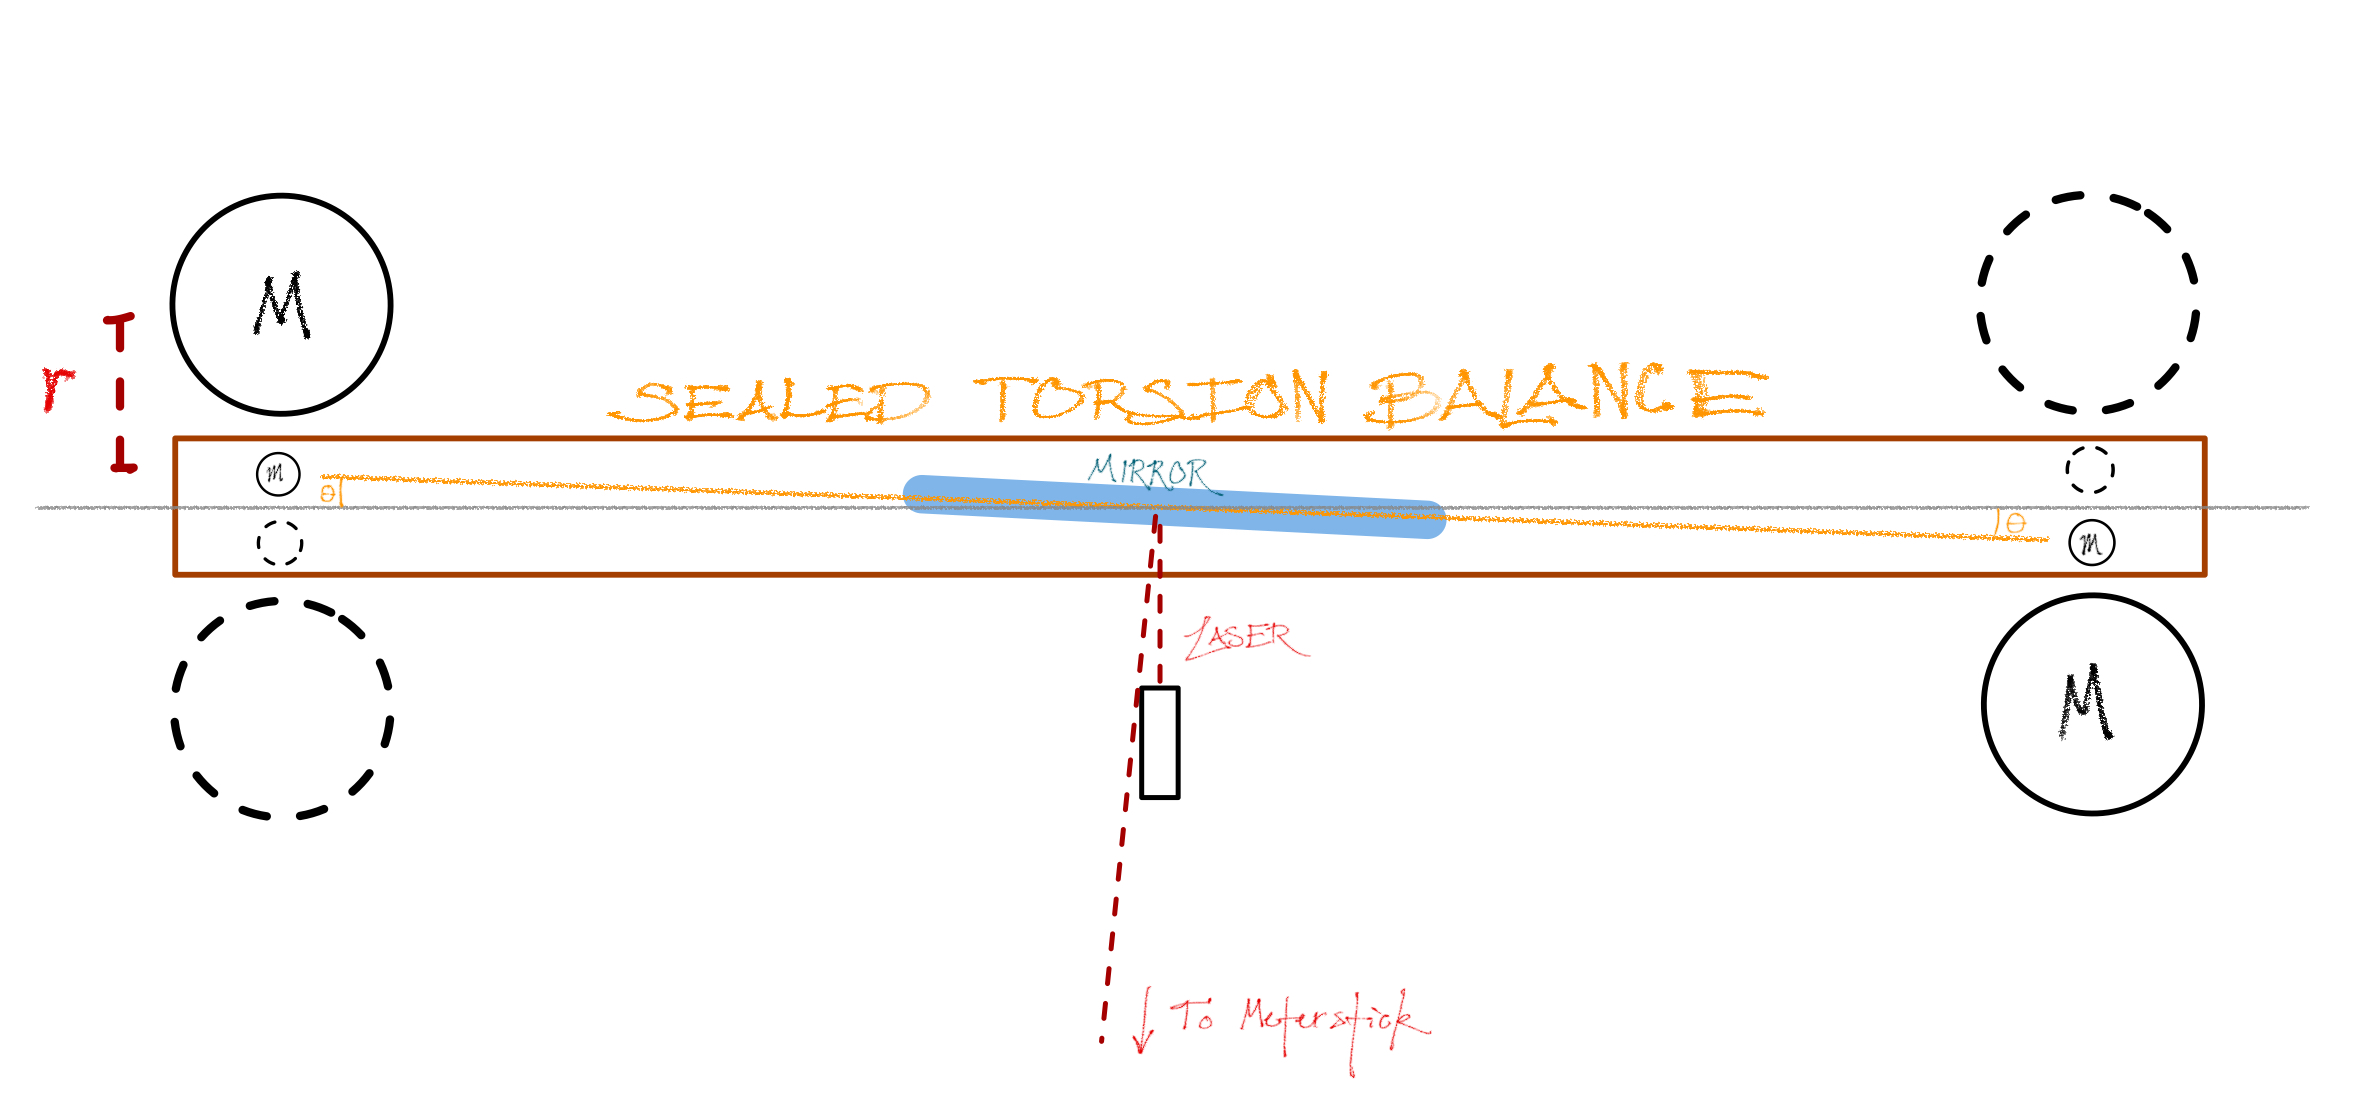
\includegraphics[width=\linewidth]{balance.jpeg}
      \caption{Birds-eye illustration of the sealed torsional balance system and associated weights. Notable components include both the small and large lead masses \(m\) and \(M\), a reflective mirror attached to the central portion of the torsional balance beam, and a laser light which is reflected across the room to a measuring stick. }\label{balance}
    \end{subfigure}
    \vspace{1px} % Adjust vertical spacing as needed
    \begin{subfigure}[tbh]{\linewidth}
      \centering
      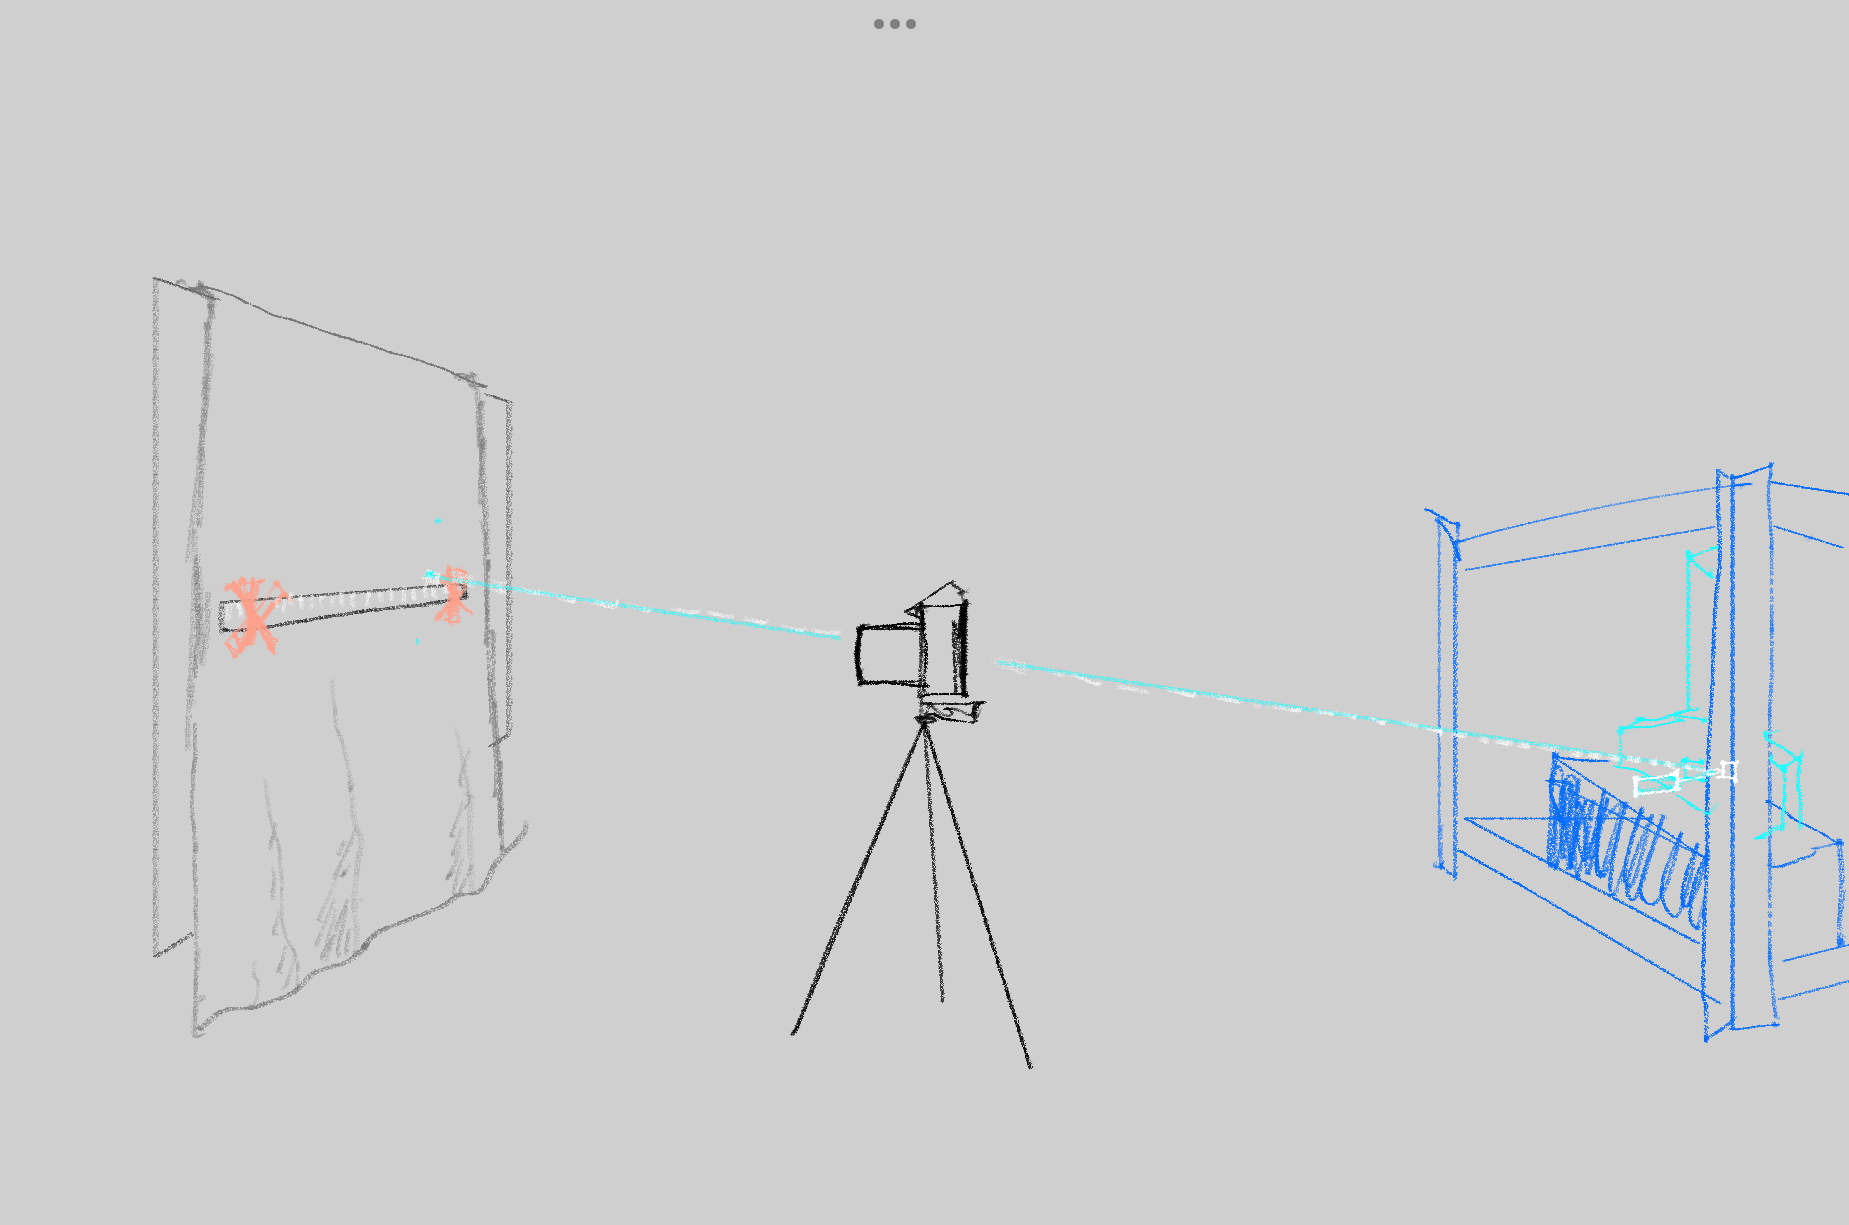
\includegraphics[width=\inverseGoldenRatio\linewidth]{board.jpeg}
      \caption{Illustration depicting measurement. A camera (center) and meter stick (left, at a known distance) were used to capture the positon of laser light reflected from the mirror affixed to central axis of the torsional balance (right, and shown in figure~\ref{balance}).}\label{board}
    \end{subfigure}
    \caption{Two sketched views of the Cavendish apparatus. Figure~\ref{balance} shows components associated with torsional balance system, while figure~\ref{board} depicts components associated with measurement.}\label{apparatus}
\end{figure}

Firstly, we mounted our meter stick on a board about 5 meters from the torsional balance's central axis, orienting said board roughly parallel with the plane of the balance's central mirror, recording the distance between the board and central axis of the balance (with uncertainty estimates).
Next, a camera was set up to take photos of the board (and the incident laser light) every 20 seconds for a duration of 90 minutes—as soon as the large lead masses were positioned.
A series of pulleys (not shown in diagram) were then used to slowly position the large lead masses (first clockwise) near the torsional balance, thereby changing the balance's equilibrium via gravitational forces.
Once the masses were in place, the camera began recording the laser position at the specified interval.
After the 90 minute duration elapsed, we repositioned the large masses, this time rotating them counterclockwise and again recording the balance's movement via the reflected laser light for the same duration.
The laser light may be turned on at any time prior to the beginning of data taking.

Laser light recorded from both orientations of the large masses was tracked digitally using an open-source tracking software, which allowed us to measure the horizontal movement of laser light associated with oscillation of the torsional balance. 
The software's main deliverable for our purposes was a set of timeseries data representing the horizontal displacement of the laser light as a function of time. 
From this timeseries data, we extracted the period and equilibrium of the oscillations for both mass orientations. In an Excel spreadsheet, we calculated \(G\) using expression~\ref{G}.
}

\section*{Results and Discussion}
{
    Using equation~\ref{G}, we found \(G\) to be about \SI[separate-uncertainty=true]{7.354 (.084) E-11}{\newton\meter\squared\per\square\kilogram}, which is within (how many \(\sigma\)?) of the accepted value of \SI{6.022E-11}{\newton\meter\squared\per\square\kilogram}. 
    With an experiment that is reliant upon the influence of such a small force, it is easy for sources of error to become overwhelming, even those that are extremely small or imperceptible. 
    It is possible that the extrema positions for the lead masses were asymmetric (\textit{i.e.} the distance \(r\) between the large masses and the torsion balance masses was not equal between the two trials). 
    Also, the presence of nearby objects, especially massive or proximal ones like people (or elevators, in our case), can introduce a great degree of unpredictability to the system.
}

% \spacing{1.2}
\printbibliography{}

\end{document}